
\documentclass[prodmode,acmtecs]{acmsmall} % Aptara syntax
% \documentclass[a4paper,10pt]{scrartcl}  
\usepackage{graphicx, incgraph,tikz,pdfpages}  


% Package to generate and customize Algorithm as per ACM style
\usepackage[ruled]{algorithm2e}
\usepackage[utf8]{inputenc}
\renewcommand{\algorithmcfname}{ALGORITHM}
\SetAlFnt{\small}
\SetAlCapFnt{\small}
\SetAlCapNameFnt{\small}
\SetAlCapHSkip{0pt}
\IncMargin{-\parindent}


\vbadness=10000
\hbadness=10000


% Metadata Information

% Copyright

% DOI

%ISSN

% Document starts
\begin{document}
	
% Title portion
\title{Optimizing asset allocation with a multiagent approach}
\author{LUCAS OLIVEIRA SOUZA
	\affil{Universidade de Brasília}
}

% Page heads
\markboth{Oliveira Souza, Lucas}{Optimizing asset allocation with a multiagent approach}

\begin{abstract}

	In 2013 Eugene Fama won the Nobel Prize for Efficient Market Hypothesis, which states that all relevant information regarding a company is already contained in its stock price, having no possibility therefore for prediction of stock price trends. That assumption has been challenged for many decades, but it has gained new colors with the rise of data science and machine learning as research field.
	
	This paper builds upon the latest research to build a multiagent system to solve the optimal asset allocation problem, aiming to maximize return of an investment porfolio. Several AI methodologies are used along, including multiple non linear regressors to predict stock price trends, such as neural networks and support vector regressors, and model-based reinforcement learning methodology Q-learning on historical data to improve the stock trading policy.

\end{abstract}

\ccsdesc[300]{Computing methodologies~Machine Learning methodologies, Multiagent systems}
	
\terms{Artificial Intelligence, Multiagent Systems}

\keywords{Artificial Intelligence, Multiagent Systems, Neural Network, Non Linear Regressors, Stock Price, Stock Market, Assets Allocation, Portfolio Optimization}

\maketitle

\section{Introduction}

Choosing to buy assets based on a predictive upward trend a discipline that dates back to the early days of capitalism. In 1637, in Holland, there was a non expected surge in tulips prices due to speculation, that caused a tulip bubble which today is widely regarded as the first “stock market crash”. The bubble was caused by investors buying tulips with the expectation that its price would raise in the long term. 

These events are more frequently in the last 30 years due to the introduction of computing intelligence in the stock trading game. Technical analysts have tried to predict future trends solely based on price and volume historical data, using esoterica methodologies of charts interpretation that even includes Leonardo da Vinci’s infamous golden ratio. Fundamental analysts have manipulated millions of spreadsheets to come upon the perfect expected price of the company and based on it predict whether its price would raise or fall.

More recently, we have seen the introduction of artificial intelligence methodologies in investment portfolio management. The rise of machine learning has drawn a lot of interest to this field, which promises big rewards for those who can crack the challenge.

When a bank or a hedge fund decides which stock to buy and which to sell, many players are involved in the decision. There are those who gather the data, those who process it and try to come up with stock price trends, and those who use this information to trade.

The multi agent approach that follows is based on this pattern encountered in real day-to-day trading. Each agent is a reflection of a role that would be occupied by an employee in a hedge fund organogram. The behavior of each agent is heavily based on artificial intelligence methodologies, such as supervised learning and reinforcement learning, which inputs intelligence into the designed system.

\section{Literature Review}

Hafezi, Sharabi and Havadandi [1] details a multi agent systems for stock price prediction. The architecture presented by the authors is a four-layered architecture, in which the first layer collects the data from various sources, both qualitative and quantitative, the second layer preprocess the data, the third layer predict the prices using a bat neural network, and a fourth layer that generates scenarios based on the prediction generated and present report to the decision makers. Only the middle two layers were implemented, with the remaining cited as future work. 

Similar approaches are found in previous works [2, 9]. While the earlier is focused on on predicting stock prices trend, the later are more concerned with investment decisions that optimize asset allocation. Lee et al. [2] implements a multi agent system that uses reinforcement learning for the trading agent, along with traditional strategies for predicting stock price. He argues that given enough time and data a non-parametric machine learning method can discover complex non-linear relationship that makes the market predictable, and invalidate the Efficient Market Hypothesis. Its system is based on previous works on applying Q-learning, recurrent  reinforcement learning and adaptive reinforcement learning to stock trading [3, 7, 8].

Vast literature is available on the topic of using non-linear regressors to predict stock prices. There seems to be a concentration in neural networks, considered to be the state of the art in non-linear regressors, as discussed by Nemes and Butoi [6], Reza et al. [1] and Chenoweth et al. [4]. Neural networks is a popular algorithm since the 70s, and since them several algorithms have been designed with the same basis but slight variations, such as convolutional neural networks and deep belief networks.

The designed systems have been applied to a variety of markets, from Romania [6] to Germany [1] to Brazil [10]. This article focuses exclusively on assets traded in Brazilian stock market Bovespa, although there are no limitations to expand to other markets and other types of assets rather than company stocks.

\section{Multi-agent architecture} 

The starting point of defining a multi-layer agents architecture is setting its goal and subgoals. The greater goal of the system in this case is to maximize the return of the portfolio, and one the relevant subgoals is to achieve accuracy in predicting future stock price.

The architecture is a two pass vertically oriented multi agent architecture. The portfolio optimization layer receives input from the user of which assets to consider, how much capital to allocate and a timeframe, and outputs buy and sell orders. The data gathering layer also communicates with the world to collect data available online, using html scrappers and relevant APIs. 

\begin{figure}
	\centering
	\includegraphics[scale=.5]{architecture}
	\caption{Multiagent Architecture}
	\label{fig:one}
\end{figure}

The three layers represent crucial steps in the assets optimization strategy. Differently from other architectures proposed [1], the feature selection step is done in conjunction with the regression, by the same agent. This is required due to the use of different non linear regression algorithms, of which some benefit from the use of more features, like decision trees and neural networks, while others require a smaller but more relevant set of features, such as a support vector regressor.

\section {Data Gathering} 

The data gathering is done using only public available data, to ensure repeatability. There are several agents contained in this step, of which I will highlight the most relevant ones.

\subsection {Price and Volume} 

Price and Volume data is obtained mainly from Yahoo Finance API and Bovespa website, that makes the data available through position based text files after the stock market closed. Since the data is updated on a daily basis, only strategies based swing trading (tradings within the week) or longer period are available. 

To execute strategies based on arbitrage, that requires information from buy and sell orders, or day trading, that requires intraday data, we would need to access a paid provider, which is not within the scope of this project.

\subsection {Twitter}

Twitter is a major force of information world wide, but it is not widely used Brazil specially related to professional aspects. Nevertheless, the data is easily accessible through a friendly API and has shown relevance in stock market prediction performance. The data is filtered through a sentiment analysis algorithm. A well trained sentiment analysis algorithm requires massive dataset, and it is not the purpose of this project to do it that. Hence, public available APIs for sentiment analysis are used (currently HP Haven) to classify the twitters into positive or negative.

\subsection {News}

News are also easy to come by and can have a great impact. News are harder to classify than Twitter, which only contains 140 characters, but have greater insight amongst them. Using news to properly predict trends in stock prices is commented on many articles [1,6], but few implementations are available due to the challenges of automatic extracting information from long elaborated texts. 

\subsection {Technical Indicators}

Technical indicators have been used since early 20th century to predict stock price trends, with some success. There is a discussion whether their performance is based on their predictive power or a self-realized prophecy - if everyone thinks a stock price will raise, that will increase the demand, and therefore increase the stock price as well. Nevertheless, the fact is they are effective and our tests have shown that indicators have a significant correlation with future stock prices.

Indicators emit a buy and sell signal at some points. For example, in a Bollinger Bands strategy, a buy signal is emitted when the stock prices touches the lower band, and a sell signal when it touches the upper band. The lower and upper bands corresponds to the value of two standard deviations above or below the moving average mean of the stock price. It can be a moving average from any number of days, depending on the timeframe of the stock trades. In the visualization below, we are using 20 days Bollinger Bands, and examples of buy and sell signals are circled in red:

\begin{figure}
	\centering
	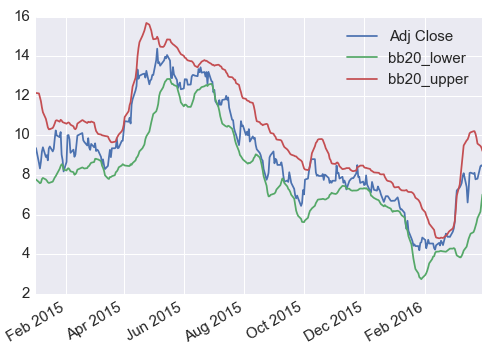
\includegraphics[scale=.5]{bbfig}
	\caption{Buy and Sell signals with a 20 days Bollinger Band}
	\label{fig:two}
\end{figure}

Another common strategy is the use of multiple moving averages. A moving average represents the true price of the stock by smoothing the daily peaks and valleys that result from speculation. When a 20 day moving average moves upwards and reaches a 50 day moving average, the interpretation is that the uprising is not only due to speculation but it has reached the point that will have a positive impact on the long term price trend for the stock, so it emits a buy signal. The same is true for the opposite, when a 20 day moving average moves downwards and it reaches a 50 day moving average it emits a sell signal. The visualization shows this in the same stock and period of the visualization above, with examples of buy and sell signals circled in red:

\begin{figure}
	\centering
	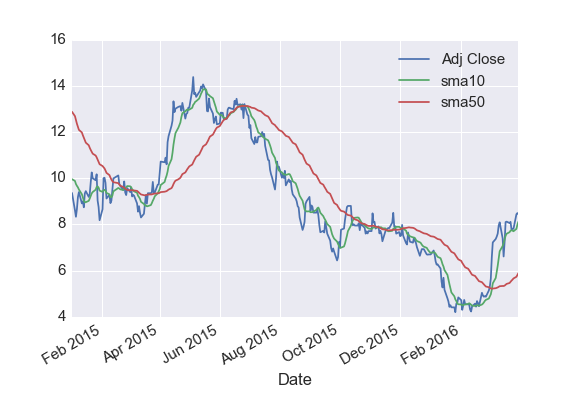
\includegraphics[scale=.5]{smafig}
	\caption{Buy and Sell signals with 20/50 days Moving Averages }
	\label{fig:three}
\end{figure}

More popular indicators are Japanese Candlesticks, and Elliot Waves, which are used in several work related to stock price predictions [4, 11] . There are number of other indicators, which go way beyond 300, well documented within books and articles of technical trading. It is time consuming to calculate buy and sell signals, so we focus on only a few of them which have higher status in the technical trading community and leave the other for future implementations. Apart from those mentioned, we have also implemented Momentum and Daily Returns.

\subsection {Fundamental Indicators}

Fundamental indicators aim to predict the true price for the stock based on public available data for the company, such as Quarterly Revenue, Number of Employees and Assets/Liabilities ratio. The general idea is that a stock price will oscillate due to speculation, but it always return to their true price. The goal of an investment analyst then is to calculate the true price of a stock based on the company’s available information, and emit a buy or a sell signal based on the difference of the true prices versus the actual price of the stock.

Fundamental indicators are harder to come by, since they are not only based on Price and Volume data. Some finance websites gather information, such as Bloomberg and Yahoo Finance. The data currently used is based on Yahoo Finance API and it uses two main indicators: EPS, Earnings Per Share, which is the amount of profit allocated to each share; and P/E, Price Earnings Ratio, the measure of its current share price relative to its per-share earnings.

More general indicators are captured to get an overall trend of the market, including: Selic Rate, which is the basic interest rate in Brazil, Working Capital Rate, which is the average interest rate for working capital. Other economical indicators not currently used but could be correlated with the overall trend is unemployment , saving loans rate and monthly expected inflation.

\section {Data Wrangling}

All this data collected would be useless if they could not be converted to features for the machine learning regression phase. That is done by a Data Wrangling agent, that acts like a manager in this phase. Its communication with the other agents is by an Request-Inform protocol. The Data Wrangler agents receives from the above layer the requirement of which period to collect data from and what are the available assets, and based on it sends a request to the Scrapper agents. Upon receiving the data, it converts them to features.

The process of converting to features is a preprocessing step in the machine learning pipeline. In this step, categorical data is converted into numerical data (and converted back to evaluate the results later). All values are normalized to fit within a expected range, so the importance of the feature to the algorithm is not influenced by the numerical scale of the variable. In this work, we are using a minmax standardization algorithm, which is given by the following formula:	 

\begin{figure}
	\centering
	\includegraphics{minmaxstandard}
	\caption{Normalizing features}
	\label{fig:four}	
\end{figure}

\subsection {Stock Price Prediction}

While there is very little information on data gathering process, a lot has been written about predicting stock price trends using machine learning algorithms [1,4, 5]. A common option is neural networks, which is considered the state of the art algorithm for non linear regression (neural networks are commonly used for classification, but it can also be applied for regression or unsupervised learning). 

Neural networks is a field of study within itself and is referred to as deep learning. There are a lot of variations of neural network architectures, most of them based on nature, such as convolutional neural network, based on how the visual cortex processes signals, and a bat neural network, which is based on the behavior of sonars that bats used to echolocate in an environment.

Nevertheless, there are other interesting non-linear regressor algorithms which bring similar results. Decision trees have the advantage of being easily interpreted, and it helps on deciding which features to keep and which to discard, generating a valuable feedback for the data gathering layer. Support vectors also have their own variation called support vector regressors which have been implemented with good results. 

\subsection {Data Analysts}

Each data analyst in this layer is responsible to predict stock prices using a pre-defined algorithm, which defines its role. All of them have access to the same information generated by the data gathering layer, and it is provided by the Data Manager.

The communication between Data Manager and Data Analyst is done by a contract-proposal protocol, similar to Contract Net protocol [11]. The Data Manager issues a call for proposal to all data analysts, providing the information of stocked and period. The data is made available in a common repository accessed by all parts, which avoid using more bandwith in the communication between the manager and analysts.

The Data Analyst attempts to predict the stock price, and evaluate its performance using backtesting. Backtesting is an approach to cross validate time series data. It trains the data within a timeframe, let’s say n-months, make predictions for m months after this period, and then evaluate its performance based on the accuracy of the predictions. In backtesting the data can not be randomized or shuffled; it is important to keep the sequentiality of the data. 

The results of the backtesting are sent to the Data Manager for evaluation. The Manager chooses the best results, and awards the winner based on it. The results from the regressor algorithm that won the proposal will be submitted to the next layer and be used to optimize the asset allocation process.

\subsection {Data Manager}

Apart from what has been described about the Data Manager, it is important to notice that it acts upon request from the next layer, the Portfolio Optimization. The input of which stock to predict and what period is given by the Fund Manager, and the results also return to it, using a Request-Inform protocol.

\section {Portfolio Optimization}

The last layer is the most relevant and represents the main goal of the overall system: to optimize asset allocation within a portfolio and maximize investment return. The approach proposed in this layer is unique regarding to the use of multiple strategies in a multi agent approach, and has not been found parallel in published articles. 
Fund Manager

A Fund Manager is the point of communication with the outside world. It receives an input of how much capital it will be allocated, a time period, and which assets should be considered (for example, we can trade high liquidity stocks in Bovespa, which is a restricted scope, or all stocks in Latin America stock markets).

The Fund Manager sends a call for proposal for all investment analysts with the above cited requirements. The stock price prediction data, made available in the last layer, is shared through a common repository that avoids overuse of the communication channel and reduces bandwith requirement. 

\subsection {Investment Analysts}

Investment Analyst carry the main burden, to optimize allocation asset. It has a pre-defined strategy that differentiates one agent from another. A few of these strategies are discussed in this article, but there is room to implement more strategies based on more elaborate strategies such as using stock options to maximize return on amount of capital invested. 

Investment analysts have access to the data produced by data analysts in the previous layer, a prediction of future stock prices. Its strategy is applied to the predictions of future trends, not only to current data on the stock, which gives it a competitive advantage over naive players in the market, such as individual investors.  

The strategy is refined through a model-free reinforcement learning strategy. In this system we are using Q-Learning, which have shown good results in previous works when applied to portfolio optimization [3]. The agent learns by applying its strategy to past data, which is similar to a backtesting strategy with the addition of a learning component. 

After converging to an optimal policy, the agent applies to the requirements given by the Fund Manager. The output to the Fund Manager is not which stocks to buy, but rather which policy to follow. That policy is to be applied by the Fund Manager throughout the period of investment, making use of online learning to keep the policy updated. 

\subsection {Buy and Hold}

The most common strategy in portfolio investment (and advertised by billionaires such as George Soros and Warren Buffet) is the buy and hold strategy. That simple entails that you pick your stocks well based on long term trends and hold it until another better opportunity appears. Short term price fluctuations are not taken into account and viewed simply as speculation. Business news and major changes in the fundamental indicators are more important buy and sell signals than technical indicators based on price and volume

\subsection {Swing Trading}

Swing trading entails buying and selling stocks within the week period (there are variations within the investment community, but one week is a commonly used timeframe). The goal is to start and end the week with no stocks in portfolio, and with the capital higher than started. Swing trading is a variation from day trading, and it is more applicable to this scenario where are using daily fluctuations and not intraday fluctuations to predict stock price trends.

\subsection {Risk Taker}

A risk taker is a strategy based on the Capital Asset Pricing Model. The CAPM methodology states that every asset has two components that determine its price, beta and alpha. 

Beta states how much of the price is determined by the overall market. An asset with a beta of 2 means that every time the market goes up 1\% the stock will go up to 2\%. In the same manner, a beta of -1 means that if the market goes up 1\% the stock will go down 1\%. Alpha, on the other hand, is how much of the price change is particular to the peculiarities of the stock and not shared with the market. 

A risk taker will look for stocks with high Beta, either positive or negative, and maximize its return on market fluctuations, exposing itself to a high risk based on the confidence it has on the stock price predictions.

\subsection {Day Trader}

A day trader goal is to start and end the day with full liquidity, buying and selling assets in the intraday market. It has not been implemented due to the lack of intraday data

\subsection {Other Strategies}

There are a lot of different strategies that can be applied by agents. A common one in hedge funds is arbitrage, that takes advantage of differences in the official stock price and the prices listed in the buy and sell order books. There are also multiple strategies involving derivatives and futures, such as stock options, which could be useful to maximize return over investment when there is high confidence in the stock price prediction.

Other strategies include also blue caps and small caps trading, which refer to buying and selling assets with high liquidity or with low liquidity. Assets known as small caps usually have a high return but high risk, since you can not always sell the stock at the moment you expect due to low liquidity, while blue caps favor from high liquidity and are better for short term trades.

\subsection {Reporting}

The Fund Manager communicates with the outside world through a reporting layer. The reporting layer is simple, and it contains only what stocks to buy, the amount and when. In this work we will not implement automatic trading, as it is a requirement of difficult implementation in Brazilian market which demands infrastructure beyond the available means. Hence, the trading orders needs to be carried on by a human investor by using the home broker of choice. 

\section {Challenges}

\subsection {Lag Selection}

One of the most discussed aspects of feature selection in time series data is the lag selection [1]. You can use all data available toda to predict stock prices one day in the future, two days, or n days. Generally, the far you move from the present day you add more noise to the prediction data. 

But some features may have a better prediction power for the stock price five days ahead than in the next day. The reason for this is that in the longer term the stock price represents its actual price, while in the shorter term the data suffers from a lot of variance from speculation. 

For each feature, then, we must apply a lag selection protocol that test different lag periods to evaluate for which n, n being the number of days ahead, the feature will maximize its prediction performance. Lag selector applied to a large number of features requires heavy computational power, both regarding to memory and processing, and it is a challenge when implementing prediction of time series data.

\begin{figure}
	\centering
	\includegraphics[scale=.5]{lagselection}
	\caption{Sample of prediction for n days ahead, using Multilayer Perceptron with 10 hidden layers}
	\label{fig:one}
\end{figure}

\subsection {Technical Trading Signals}

Technical trading signals are hard to calculate. Each agent has a complex implementation. The challenge is to implement a procedure that generates buy and sell signals based on the indicator axioms. This is usually done by a human analyzing charts, but it needs to be converted into a programmatic procedure.  As with the lag selection, calculating technical trading signals is consuming both in terms of memory and processing. 

\subsection {Data Gathering}

The process of gathering online available data is easy to carry once implemented, but it requires a significant bandwidth in order to attend to time requirements in the system. For example, in a swing trading strategy, trading is done on weekly basis, which requires massive data gathering and processing before the beginning of every week. 

\section {Implementation}

The implementation make use of several open source Python packages freely available on the web. Scikit Learn [12] is used for machine learning algorithms and data preprocessing features. Pandas [13] and matplotlib [14] are used for data wrangling and visualization. Seaborn [15] generates interesting covariance matrixes that are useful to analyze the features.

The agents implementation is done with the assistance of SPADE [16], Smart Python Agents Development Environment, which is FIPA-compliance implementation of a multi agent environment based on JADE.

Rodeo and Jupyter Notebooks [17] are python IDEs customized to data manipulation and machine learning. The infrastructure used is a local Mac notebook, with 8 cores and 16gb ram. Future implementations will be based on Amazon Elastic Search for better scalability.

Much of the work described is still at the architectural level, and it requires a few months of work to be a fully tested system. While there is a temptative implementation, no significant results have been achieved that would justify publishing. 

\section {Conclusion}

Stock trading can be seen as the most complicated game of all, played by millions of capable humans, and with huge rewards at a stake. It can be considered the ultimate challenge for an AI. If an autonomous agent can have a significant competitive advantage over other players in the stock market, it will become capable of raising capital to pursue its goals.

That raises questions on the security of automatic trading in the stock market. There has been numerous episodes of market crash, with a significant impact of the economy, due to poor management of automatic trading strategies by large banks and hedge funds. 

The concern is even bigger if we take into consideration that most of the research in the area is done privately and kept unpublished. While there are published articles in the field, it is clear that the results achieved by those that publish their work is not the state of the art in the field, which is practiced inside closed doors at investment boutiques, hedge funds and banks.

It is important that the academia takes on the challenge. It would benefit from the advancements that come from applying AI to a difficult challenge, and avoid the higher risk of having one player with an ultimate competitive advantage of other players, which can lead to catastrophic results.

This research, while still lacking publishable results, suggests the use of a wide range of AI techniques to optimize assets allocation in an investment portfolio. Its proposals are built from previous work by many researchers, and as such, makes its own contribution to the advancement of the applied artificial intelligence field of study.

\section {References}

\begin{enumerate}

\item Hafezi, R., Shahrabi, J., \& Hadavandi, E. (2015). A bat-neural network multi-agent system (BNNMAS) for stock price prediction: Case study of DAX stock price. Applied Soft Computing, 29, 196-210.

\item Lee, J. W., Park, J., Jangmin, O., Lee, J., \& Hong, E. (2007). A multiagent approach to Q-learning for daily stock trading. IEEE Transactions on Systems, Man, and Cybernetics-Part A: Systems and Humans, 37(6), 864-877.

\item Gao, X., \& Chan, L. (2000). An algorithm for trading and portfolio management using Q-learning and sharpe ratio maximization. In Proceedings of the international conference on neural information processing (pp. 832-837).

\item Chenoweth, T., Obradovic, Z., \& Lee, S. S. (1996). Embedding technical analysis into neural network based trading systems. Applied Artificial Intelligence, 10(6), 523-542.

\item Rahimi, S., Tatikunta, R., Ahmad, R., \& Gupta, B. (2009). A multi-agent framework for stock trading. International Journal of Intelligent Information and Database Systems, 3(2), 203-227.

\item Nemes, M. D., \& Butoi, A. (2013). Data mining on romanian stock market using neural networks for price prediction. Informatica Economica, 17(3), 125.

\item Dempster, M. A., \& Leemans, V. (2006). An automated FX trading system using adaptive reinforcement learning. Expert Systems with Applications, 30(3), 543-552.

\item Moody, J., \& Saffell, M. (2001). Learning to trade via direct reinforcement. IEEE transactions on neural Networks, 12(4), 875-889.

\item Luo, Y., Liu, K., \& Davis, D. N. (2002). A multi-agent decision support system for stock trading. IEEE network, 16(1), 20-27.

\item Jabbur, E., Silva, E., Castilho, D., Pereira, A., \& Brandão, H. (2014, August). Design and evaluation of automatic agents for stock market intraday trading. In Proceedings of the 2014 IEEE/WIC/ACM International Joint Conferences on Web Intelligence (WI) and Intelligent Agent Technologies (IAT)-Volume 03 (pp. 396-403). IEEE Computer Society.

\item Wooldridge, M. (2009). An introduction to multiagent systems. John Wiley \& Sons.

\item "scikit-learn: machine learning in Python — scikit-learn 0.16.1 documentation", Scikit-learn.org, 2016. [Online]. Available: http://scikit-learn.org/.

\item "Python Data Analysis Library — pandas: Python Data Analysis Library", Pandas.pydata.org, 2016. [Online]. Available: http://pandas.pydata.org/.

\item "matplotlib: python plotting — Matplotlib 1.5.1 documentation", Matplotlib.org, 2016. [Online]. Available: http://matplotlib.org/.

\item "Seaborn: statistical data visualization — seaborn 0.7.1 documentation", Web.stanford.edu, 2016. [Online]. Available: https://web.stanford.edu/~mwaskom/software/seaborn/.

\item "SPADE 2.2.1 : Python Package Index", Pypi.python.org, 2016. [Online]. Available: https://pypi.python.org/pypi/SPADE.

\item "Project Jupyter", Jupyter.org, 2016. [Online]. Available: http://jupyter.org/.

\end{enumerate}

% End of v2-acmsmall-sample.tex (March 2012) - Gerry Murray, ACM
\end{document}